\chapter{DAC Passive Reconstruction Filter} \label{App:DAC_PASSIVE_FILTER}
This appendix will show the method used to estimate the passive DAC filter. 

The pass-band $f_p$ is desired to be at \SIQ{1.5}{\mega\hertz}, this results in a frequency scaling factor $k_f$ of $k_f = 2\pi\cdot1.5e6 = 9.4248e6$. The filter is designed such that the load impedance of the filter is the \SIQ{50}{\ohm} resistor used to convert the DAC current to a voltage. This indicates that the impedance scalign factor is $k_z = 50$.

Using nothing more than these two values, a filter can be designed by a standard LC table for a normalized low-pass Butterworth filter such as shown in figure \ref{fig:app_DAC_LC_TABLE}. A 4th order filter sets the normalized values to $L_1 = 1.5307$, $C_2 = 1.5772$, $L_3 = 1.0824$, $C_4 = 0.3827$.

\begin{figure}[H]
    \centering
    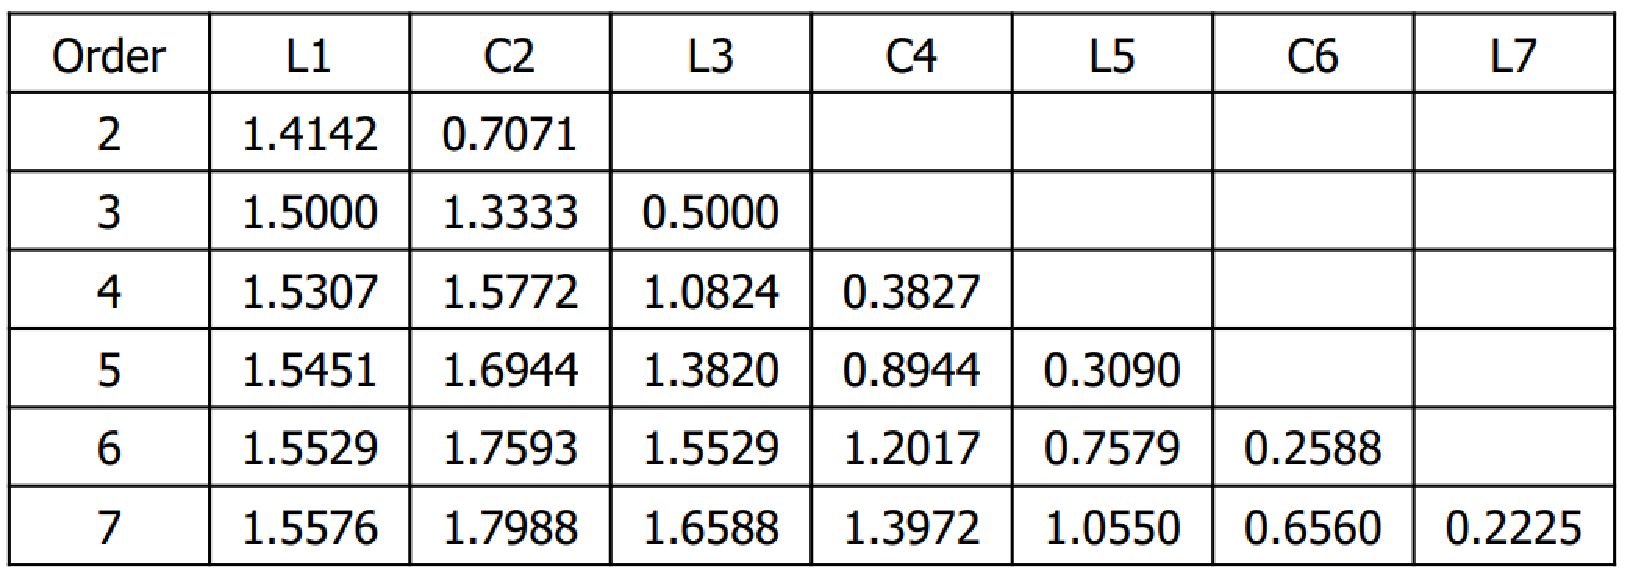
\includegraphics[clip, trim=0 0 0 0, width=1\textwidth]{Appendix/Figures/Butterworth_LC.pdf}
    \caption{Standard normalized low-pass Butterworth LC table.}
    \label{fig:app_DAC_LC_TABLE}
\end{figure}

Using the frequency and impedance scaling factor, component values can then be found. This can be seen in equation \ref{eq:app_DAC_1}.
\begin{equation}
\label{eq:app_DAC_1}
\begin{split}
    L_1 &= \frac{k_z}{k_f}1.5307 \Rightarrow L_1 = \frac{50}{9.4248e6}1.5307 = \SIQ{8.12}{\micro\henry}\\
    C_2 &= \frac{1}{k_z k_f}1.5772 \Rightarrow C_2 = \frac{1}{50\cdot9.4248e6}1.5772 = \SIQ{3347}{\pico\farad} \\
    L_3 &= \frac{k_z}{k_f}1.0824 \rightarrow L_3 = \frac{50}{9.4248e6}1.0824 = \SIQ{5.74}{\micro\henry}\\
    C_4 &= \frac{1}{k_z k_f}0.3827 \Rightarrow C_2 = \frac{1}{50\cdot9.4248e6}0.3827 = \SIQ{812}{\pico\farad} \\
\end{split}
\end{equation}

These exact values where not available, the used values are as in equation \ref{eq:app_DAC_2}.
\begin{equation}
    \label{eq:app_DAC_2}
    \begin{split}
        L_1 &= \SIQ{8.2}{\micro\henry}\\
        C_2 &= \SIQ{3300}{\pico\farad} \\
        L_3 &= \SIQ{5.6}{\micro\henry}\\
        C_4 &= \SIQ{820}{\pico\farad} \\
    \end{split}
    \end{equation}



